\documentclass[serif]{beamer}
\usepackage[UTF8]{ctexcap}
\usetheme{Antibes}
\usecolortheme{beaver}

\newtheorem{thm}{定理}
\renewcommand\proofname{\heiti 证明}

\usepackage{pgfplots}
\pgfplotsset{compat=1.15}
\usepackage{mathrsfs}
\usetikzlibrary{arrows}
\newcommand{\degre}{\ensuremath{^\circ}}

\usepackage{enumitem}


\title{\textbf{\heiti 半角公式与一元二次方程}}
\author{\kaishu 程昊一}

\begin{document}
\begin{frame}
	\maketitle
\end{frame}

\part{\heiti\hspace*{\fill}\hspace*{3cm}知\hspace{\fill}识\hspace{\fill}讲\hspace{\fill}解\hspace{\fill}\hspace{3cm}}

\begin{frame}
	\partpage
\end{frame}

\begin{frame}{\heiti 目录}
	\tableofcontents
\end{frame}

\section{\heiti 一元二次方程}

\begin{frame}{\heiti 一元二次方程}
	一元二次方程的一般形式是
	\[ax^2+bx+c=0.\]
	后文为了方便讨论, 我们将等式两端同时除以$a$, 记$p=b/a$, $q=c/a$, 于是得到
	\begin{equation}
		x^2+px+q=0.\label{eq:basic}
	\end{equation}
\end{frame}

\subsection{\kaishu 分步探索}

\begin{frame}{\kaishu 分步探索}
	假设我们的方程(\ref{eq:basic})有两个根$s$与$t$, 我们有
	\[\begin{cases}
		s^2+ps+q=0\\
		t^2+pt+q=0
	\end{cases}\]
	两式相减并稍作整理, 得到
	\[(s-t)(s+t+p)=0.\]
\end{frame}

\begin{frame}
	考察$-(p+s)$. 代入方程(\ref{eq:basic}), 发现方程也成立. 那么, 无论如何, $-(p+s)$也是方程的根.\par
	而且, 容易证明(反证法), 方程(\ref{eq:basic})至多有两个根(重根不算做多个). 那么我们有理由相信:
	\[t=-(p+s).\]
	于是我们得到了一个结论:
	\begin{block}{{\heiti 命题}\textbf{1}}
		\kaishu
		对于方程(\ref{eq:basic}), 若$s$为其根, 则
		\[t=-(p+s)\]
		也为其根, 并且至多有两个根.
	\end{block}
\end{frame}

\begin{frame}
	\begin{proof}
		\vspace*{6cm}
	\end{proof}
\end{frame}

\begin{frame}
	什么时候两根相等呢?
	我们列方程$s=t$, 即
	\[s=-(p+s),\]
	得到
	\[s=t=-\frac{p}{2}.\]
	代入原方程, 得到
	\[p^2=4q.\]
	我们又得到以下结论:
	\begin{block}{{\heiti 命题}\textbf{2}}
		方程(\ref{eq:basic})的两根相等的充分必要条件为
		\[p^2=4q.\]
	\end{block}
\end{frame}

\begin{frame}
	由命题1, 我们可以得到
	\begin{equation}
		s+t=-p.\label{eq:sum}
	\end{equation}
	即两根之和为$-p$. 我们想解出来$s$与$t$, 就要再找到一个$s$与$t$的关系.\par
	回到开始的方程组
	\[\begin{cases}
		s^2+ps+q=0\\
		t^2+pt+q=0
	\end{cases}\]
	两式相加, 得到
	\[s^2+t^2-p^2+2q=0.\]
	即
	\begin{equation}
		s^2+t^2=p^2-2q.\label{eq:squaresum}
	\end{equation}
\end{frame}

\begin{frame}
	于是我们得到了$s$与$t$的两个关系: (\ref{eq:sum})与(\ref{eq:squaresum}).知二求二即可, 具体过程留给大家作为习题.\par
	(提示: 可先表示出$s-t$(不妨设$s\ge t$), 结合$s+t=-p$分别解出$s$与$t$.)
\end{frame}

\subsection{\kaishu 求根公式}

\begin{frame}{\kaishu 求根公式}
	我们有如下定理:
	\begin{block}{{\heiti 定理}: {\fangsong 一元二次方程的求根公式}}
		\kaishu
		对于方程$x^2+px+q=0$, 其两根$x_{1,2}$为
		\[x_{1,2}=\frac{-p\pm\sqrt{p^2-4q}}{2};\]
		一般地, 对于方程$ax^2+bx+c=0 (a\neq 0)$, 其两根$x_{1,2}$为
		\[x_{1,2}=\frac{-b\pm\sqrt{b^2-4ac}}{2a}.\]
	\end{block}
\end{frame}

\begin{frame}
	\begin{block}{\hspace*{\fill}(续)}
		\kaishu
		其中, $p^2-4q$或$b^2-4ac$被称作二次方程的{\heiti 判别式}, 记作$\Delta$(大写希腊字母Delta). 二次方程的根的情况与判别式有如下关系:
		\[\begin{cases}
			\Delta <0\Rightarrow\text{原方程无实根};\\
			\Delta =0\Rightarrow\text{原方程有两个重根};\\
			\Delta >0\Rightarrow\text{原方程有两个不相等的实根}.
		\end{cases}\]
	\end{block}
\end{frame}

\begin{frame}
	\begin{proof}
		\vspace*{6cm}
	\end{proof}
\end{frame}

\subsection{\kaishu Vieta定理}

\begin{frame}{\kaishu Vieta定理}
	如果大家仔细推导过上面的“知二求二”, 或直接从求根公式中观察, 就会发现如下定理:
	\begin{block}{{\heiti 定理}: {\fangsong Vieta定理(韦达定理)}}
		\kaishu
		设方程$ax^2+bx+c=0(a\neq 0)$有两根$x_{1,2}$, 则
		\[\begin{cases}
			x_1+x_2=-\dfrac{b}{a}(=-p);\\
			x_1x_2=\dfrac{c}{a}(=q).
		\end{cases}\]
	\end{block}
	不难, 请大家自证.
\end{frame}

\begin{frame}{\kaishu *拓展: 一元$n$次方程的Vieta定理}
	事实上, 对于一般的一元$n$次方程, 我们也有Vieta定理. 如下:
	\begin{block}{{\heiti 定理}: {\fangsong 一元$n$次方程的Vieta定理}}
		\kaishu
		设方程$a_nx^n+a_{n-1}x^{n-1}+\cdots+a_1x+a_0=0$有$n$个根(无论是实根还是虚根)$x_{1,2,\cdots,n}$.那么有:
		\[\begin{cases}
			\sum\limits_{k=1}^{n}x_k=-\frac{a_{n-1}}{a_n};\\
			\sum\limits_{1\le k_1<k_2\le n}x_{k_1}x_{k_2}=\frac{a_{n-2}}{a_n};\\
			\sum\limits_{1\le k_1<k_2<k_3\le n}x_{k_1}x_{k_2}x_{k_3}=-\frac{a_{n-3}}{a_n};\\
			\cdots\\
			x_1x_2\cdots x_n=\frac{(-1)^na_0}{a_n}.
		\end{cases}\]
	\end{block}
\end{frame}

\begin{frame}{\kaishu\normalsize *一元$n$次方程的Vieta定理的证明}
	我把证明放在这里, 有兴趣的同学不妨一览.\par
	{\fangsong
		将原方程的左端因式分解为
		\[a_n\prod\limits_{k=1}^{n}(x-x_k).\]
	}
	
\end{frame}

\begin{frame}
	\fangsong
	展开, 得
	\begin{align*}
		\sum\limits_{k=0}^{n}a_kx^k
		=&a_n\prod\limits_{k=1}^{n}(x-x_k)\\
		=&a_nx^n
		-a_n\left(\sum\limits_{k=1}^{n}x_k\right)x^{n-1}\\
		&+a_n\left(\sum\limits_{1\le k_1<k_2\le n}x_{k_1}x_{k_2}\right)x^{n-2}\\
		&-a_n\left(\sum\limits_{1\le k_1<k_2<k_3\le n}x_{k_1}x_{k_2}x_{k_3}\right)x^{n-3}\\
		&+\cdots\\
		&+a_n(-1)^n(x_1x_2\cdots x_n)
	\end{align*}
\end{frame}

\begin{frame}
	\fangsong
	对比等式两边各项的系数, 得到
	\[\begin{cases}
		a_n=a_n\\
		a_{n-1}=-a_n\left(\sum\limits_{k=1}^{n}x_k\right)\\
		a_{n-2}=a_n\left(\sum\limits_{1\le k_1<k_2\le n}x_{k_1}x_{k_2}\right)\\
		a_{n-3}=-a_n\left(\sum\limits_{1\le k_1<k_2<k_3\le n}x_{k_1}x_{k_2}x_{k_3}\right)\\
		\cdots\\
		a_0=a_n(-1)^n(x_1x_2\cdots x_n)
	\end{cases}\]
	整理即证.\hspace{\fill}\qed
\end{frame}

\section{\heiti 正弦的半角公式}

\begin{frame}{\heiti 正弦的半角公式}
	我们熟知倍角公式
	\[\sin2\alpha=2\sin\alpha\cos\alpha.\]
	而
	\[\sin^2\alpha+\cos^2\alpha=1.\]
	这又是一个“知二求二”问题, 请大家自己完成. 下面给出一个利用二次方程推出半角公式的方法($\alpha<90^\circ$).
\end{frame}

\subsection{\kaishu 分步探索}

\begin{frame}{\kaishu 分步探索}
	假设我们已知$\sin2\alpha=k$, 设$\sin\alpha=x$, 则$\cos\alpha=\sqrt{1-x^2}$. 那么上面的倍角公式就可以写为
	\[k=2x\sqrt{1-x^2}.\]
	两边平方, 得到
	\[k^2=4x^2(1-x^2).\]
	做换元$t=x^2$, 则有
	\[k^2=4t(1-t).\]
	整理, 得
	\[4t^2-4t+k^2=0.\]
\end{frame}

\begin{frame}
	根据之前给出的求根公式, 就有
	\[t=\frac{4\pm\sqrt{4^2-4\times4k^2}}{2\times4}.\]
	在这里, 应该舍弃正号. 稍加整理, 得
	\[t=\frac{1-\sqrt{1-k^2}}{2},\]
	即
	\[\sin^2\alpha=\frac{1-\sqrt{1-\sin^22\alpha}}{2}\left(=\frac{1-\cos2\alpha}{2}\right).\]
\end{frame}

\subsection{\kaishu 一般性结论}

\begin{frame}{\kaishu 一般性结论}
	我们有如下结论:
	\begin{block}{{\heiti 定理}: {\fangsong 正弦的半角公式}}
		\kaishu
		若$\alpha$为小于$180^\circ$的角, 那么有
		\[\sin\frac{\alpha}{2}=\sqrt{\frac{1-\sqrt{1-\sin^2\alpha}}{2}}\left(=\sqrt{\frac{1-\cos\alpha}{2}}\right).\]
	\end{block}
\end{frame}

\section{\heiti *余弦的半角公式}

\begin{frame}{\heiti *余弦的半角公式}
	因为我们有
	\[\sin^2\frac\alpha2+\cos^2\frac\alpha2=1,\]
	所以
	\begin{align*}
		\cos\frac\alpha2&=\sqrt{1-\sin^2\frac\alpha2}\\
		&=\sqrt{1-\frac{1-\sqrt{1-\sin^2\alpha}}{2}}\\
		&=\sqrt{\frac{1+\sqrt{1-\sin^2\alpha}}{2}}\\
		&=\sqrt{\frac{1+\cos\alpha}{2}}.
	\end{align*}
\end{frame}

\begin{frame}
	所以我们有:
	\begin{block}{{\heiti 定理}: {\fangsong 余弦的半角公式}}
		\kaishu
		若$\alpha$为小于$180^\circ$的角, 那么有
		\[\cos\frac\alpha2=\sqrt{\frac{1+\sqrt{1-\sin^2\alpha}}{2}}=\sqrt{\frac{1+\cos\alpha}{2}}.\]
	\end{block}
\end{frame}

\part{\heiti\hspace*{\fill}\hspace*{3cm}习\hspace{\fill}题\hspace{\fill}讲\hspace{\fill}解\hspace{\fill}\hspace{3cm}}

\begin{frame}
	\partpage
\end{frame}

\begin{frame}{\heiti 目录}
	\tableofcontents
\end{frame}

\section{\heiti 习题\textbf{10.1}}

\begin{frame}{\heiti 习题\textbf{10.1}}
	\kaishu 求$\sin 22.5^\circ$与$\sin 52.5^\circ$.\par
	\songti 解:\vspace{5cm}
\end{frame}

\section{\heiti 习题\textbf{10.2}}

\begin{frame}{\heiti 习题\textbf{10.2}}
	\kaishu 如图, $E$在正方形$ABCD$的边$BC$上, $\angle EAB=15^\circ$, $M$为$AE$中点. 请观察思考$\triangle MCD$有何特点, 并论证你的判断.\par
	\songti 解:
	\begin{figure}
		\flushright
		\definecolor{uuuuuu}{rgb}{0.26666666666666666,0.26666666666666666,0.26666666666666666}
		\begin{tikzpicture}[line cap=round,line join=round,>=triangle 45,x=0.75cm,y=0.75cm]
			\clip(-0.5,-0.5) rectangle (5.5,5.5);
			\draw [shift={(0.,0.)},line width=1.2pt] (0,0) -- (0.:0.75) arc (0.:15.:0.75) -- cycle;
			\draw [line width=1.2pt] (0.,0.)-- (5.,0.);
			\draw [line width=1.2pt] (5.,0.)-- (5.,5.);
			\draw [line width=1.2pt] (5.,5.)-- (0.,5.);
			\draw [line width=1.2pt] (0.,5.)-- (0.,0.);
			\draw [line width=1.2pt] (0.,0.)-- (5.,1.3397459621556138);
			\draw [line width=1.2pt] (2.5,0.6698729810778069)-- (0.,5.);
			\draw [line width=1.2pt] (2.5,0.6698729810778069)-- (5.,5.);
			\begin{scriptsize}
				\draw [fill=black] (0.,0.) circle (0.5pt);
				\draw[color=black] (-0.23336503626662675,-0.18840972838422457) node {$A$};
				\draw [fill=black] (5.,0.) circle (0.5pt);
				\draw[color=black] (5.253859351019805,-0.22928290817779193) node {$B$};
				\draw [fill=black] (5.,5.) circle (0.5pt);
				\draw[color=black] (5.2232044661746295,5.217068299315062) node {$C$};
				\draw [fill=black] (0.,5.) circle (0.5pt);
				\draw[color=black] (-0.2946748059569779,5.217068299315062) node {$D$};
				\draw [fill=uuuuuu] (2.5,0.6698729810778069) circle (0.5pt);
				\draw[color=uuuuuu] (2.5460111896959603,0.4451245584160699) node {$M$};
				\draw [fill=uuuuuu] (5.,1.3397459621556138) circle (0.5pt);
				\draw[color=uuuuuu] (5.2742959409165895,1.3852076936681195) node {$E$};
				\draw[color=black] (1.3089010484693435,0.1385757099643145) node {$15\textrm{\degre}$};
			\end{scriptsize}
		\end{tikzpicture}
	\end{figure}
\end{frame}

\section{\heiti 习题\textbf{10.3}}

\begin{frame}{\heiti 习题\textbf{10.3}}
	\kaishu 如图, $D$为$\triangle ABC$的$AB$边上的点, $\angle B=2\angle A=72^\circ$, $\angle ADC=108^\circ$.
	\begin{itemize}
		\item[(1)] 求$AB/BC$;
		\item[(2)] 利用前一结论求$\sin 18^\circ$.
	\end{itemize}
	\begin{figure}
		\flushright
		\vspace*{-2cm}
		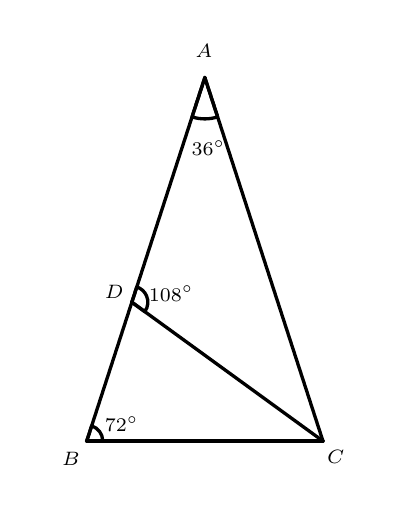
\begin{tikzpicture}[line cap=round,line join=round,>=triangle 45,x=1.5cm,y=1.5cm]
			\clip(-0.5,-0.5) rectangle (2.5,3.5);
			\draw [shift={(1.,3.0776835371752527)},line width=1.2pt] (0,0) -- (-108.:0.35) arc (-108.:-72.:0.35) -- cycle;
			\draw [shift={(0.3819660112501053,1.1755705045849465)},line width=1.2pt] (0,0) -- (-36.:0.13566443163263023) arc (-36.:72.:0.13566443163263023) -- cycle;
			\draw [shift={(0.,0.)},line width=1.2pt] (0,0) -- (0.:0.13566443163263023) arc (0.:72.:0.13566443163263023) -- cycle;
			\draw [line width=1.2pt] (1.,3.0776835371752527)-- (0.,0.);
			\draw [line width=1.2pt] (0.,0.)-- (2.,0.);
			\draw [line width=1.2pt] (2.,0.)-- (1.,3.0776835371752527);
			\draw [line width=1.2pt] (0.3819660112501053,1.1755705045849465)-- (2.,0.);
			\begin{scriptsize}
				\draw [fill=black] (0.,0.) circle (0.5pt);
				\draw[color=black] (-0.13385376182424388,-0.1540437909713695) node {$B$};
				\draw [fill=black] (2.,0.) circle (0.5pt);
				\draw[color=black] (2.1091315078352424,-0.13143305236593114) node {$C$};
				\draw [fill=black] (1.,3.0776835371752527) circle (0.5pt);
				\draw[color=black] (0.992161020726587,3.300877067939612) node {$A$};
				\draw [fill=black] (0.3819660112501053,1.1755705045849465) circle (0.5pt);
				\draw[color=black] (0.2324402035838577,1.2659105934501595) node {$D$};
				\draw[color=black] (1.03,2.4813428301506006) node {$36\textrm{\degre}$};
				\draw[color=black] (0.7146549756926251,1.2478220025658089) node {$108\textrm{\degre}$};
				\draw[color=black] (0.2960066467471207,0.14441795862041684) node {$72\textrm{\degre}$};
			\end{scriptsize}
		\end{tikzpicture}
	\end{figure}
\end{frame}

\begin{frame}
\end{frame}

\end{document}
